% ============================================================
% CAPITOLO 4 — Evoluzione topologica del grafo di mercato
% Scritto il 2026-09-13 seguendo il programma in frontmatter/abstract.tex.
% Assorbe YYY_literature-review.tex (sec:network-structure-crisis-regimes,
% sottosezione "Metriche") e ZZZ_old-case-study.tex
% (sec:topological-evolution-analysis). Decisioni di sessione:
%   - W_full, W_thresh e tau sono solo richiamati come costruiti nel Cap. 3
%     (ancora da riscrivere): nessun \cref a sezioni di ZZZ.
%   - Marchenko-Pastur: si richiama eq:marchenko-pastur del Cap. 3, qui si
%     aggiungono solo modo di mercato, entropia spettrale e bordo dello studio.
%   - Tabelle di sintesi ed event study incluse (numeri da
%     project-thesis/results/summary.md). Il 2026-09-18 sono state aggiunte le
%     tre figure di evento (grafo + heatmap affiancati, una per crisi), prodotte
%     da project-thesis/scripts/07_make_figures.py::figure_event_panels.
%   - Label con prefisso topo- per non collidere con quelli di ZZZ, ancora \input.
% ============================================================
\chapter{Evoluzione topologica del grafo di mercato}
\label{ch:topological-evolution}

Il \Cref{ch:dynamic-correlation-graph} ha trasformato i rendimenti delle quindici criptovalute in una successione di grafi, uno per ciascuna delle $1947$ finestre mobili di ampiezza $T_w=60$ giorni comprese tra il 02/03/2021 e il 30/06/2026. Per ogni finestra sono disponibili: la matrice di correlazione $C_t$, il grafo completo $W_{\mathrm{full}}$ ottenuto con i pesi di Mantegna dell'equazione~\eqref{eq:mantegna-weight} e il grafo filtrato $W_{\mathrm{thresh}}$, che conserva i soli archi con $\rho_{ij}>\tau$ per la soglia calibrata $\tau=0{,}2145$.

Questo capitolo affronta la seconda questione di ricerca posta nell'Introduzione, ovvero se la struttura del grafo si compatti nel passaggio da un regime di mercato stabile a uno di crisi. Le $1947$ finestre vengono ridotte a poche grandezze scalari, leggibili come serie temporali e calcolate dallo script \path{03_topology_analysis.py}, per semplificarne l'analisi.

\section{Misurare il compattamento del mercato}
\label{sec:topo-measuring-compaction}

La letteratura documenta, su mercati e periodi diversi, un aumento della correlazione media tra le attività nelle fasi di crisi, in coincidenza delle quali la struttura del mercato tende a compattarsi. \Textcite{onnela2003dynamics} lo mostrano seguendo nel tempo il \emph{minimum spanning tree} costruito sulla distanza di Mantegna: durante i crolli l'albero si contrae, e i titoli si dispongono più vicini tra loro anziché distribuirsi su rami lunghi. Sul versante spettrale, l'analisi delle matrici di correlazione empiriche di \textcite{laloux1999noise} individua un autovalore dominante, interpretabile come modo di mercato. Quando esso assorbe una quota crescente della varianza totale, tutte le attività si muovono di fatto insieme.

Le due osservazioni descrivono il fenomeno da due angolazioni diverse, ma nessuna grandezza, presa singolarmente, è in grado di misurarlo. Le due metriche più immediate hanno difetti complementari.

\begin{description}
    \item[Correlazione media.] È la media delle $\rho_{ij}$ sulle $N(N-1)/2$ coppie distinte. Sebbene sia semplice da calcolare e da interpretare, è di fatto cieca alla struttura. Due mercati con la stessa correlazione media possono avere legami distribuiti in modo del tutto diverso tra gli asset.
    \item[Densità del grafo.] È la frazione di archi che superano il filtraggio $\rho_{ij}>\tau$. Cresce quando il mercato si compatta, perché più coppie superano la soglia, ma dipende interamente dalla soglia scelta. Cambiando $\tau$ cambia la serie, e una soglia inadatta ai dati può appiattirla fino a renderla priva di informazione.
\end{description}

Per superare questi limiti, il caso di studio considera altre metriche, mantenendo la correlazione media e la densità come termini di riferimento.

\section{Minimum Spanning Tree (MST)}
\label{sec:topo-mst}

Uno spanning tree di un grafo connesso su $N$ nodi è un suo sottografo aciclico e connesso che tocca tutti i nodi. Ha quindi esattamente $N-1$ archi. Assegnando ad ogni coppia la distanza di Mantegna $d_{ij}$ dell'equazione~\eqref{eq:mantegna-distance}, il minimum spanning tree (MST) $T_t$ della finestra $t$ è, tra tutti gli spanning tree del grafo completo, quello di distanza totale minima. Conserva cioè gli $N-1$ legami più stretti compatibili con l'assenza di cicli.

\Textcite{onnela2003dynamics} ne riassumono la forma con la lunghezza normalizzata
\begin{equation}
\label{eq:mst-length}
L(t) = \frac{1}{N-1}\sum_{(i,j)\in T_t} d_{ij},
\end{equation}
cioè la lunghezza media di un arco dell'albero. Poiché $d_{ij}$ decresce al crescere di $\rho_{ij}$, un mercato che si compatta accorcia l'albero. La metrica non richiede alcuna soglia, perché l'MST ha sempre $N-1$ archi, e tiene inoltre conto della struttura, perché somma solo i legami che l'albero seleziona e non tutte le coppie.

Nel progetto la lunghezza~\eqref{eq:mst-length} è calcolata da \texttt{mst\_length}, che delega la costruzione dell'albero alla libreria \texttt{networkx}.

\begin{listing}[H]
\begin{minted}{python}
def mst_length(distance: np.ndarray) -> np.ndarray | float:
    distance = np.asarray(distance, dtype=np.float64)
    if distance.ndim == 2:
        return _single_mst_length(distance)
    return np.array([_single_mst_length(matrix) for matrix in distance])


def _single_mst_length(distance: np.ndarray) -> float:
    n_nodes = distance.shape[-1]
    graph = nx.from_numpy_array(distance)
    tree = nx.minimum_spanning_tree(graph)
    return sum(data["weight"] for _, _, data in tree.edges(data=True)) / (n_nodes - 1)
\end{minted}
\caption{\texttt{mst\_length} e \texttt{\_single\_mst\_length}}
\label{lst:mst-length}
\end{listing}

La funzione accetta sia una singola matrice sia l'intero tensore delle finestre. Nel secondo caso ripete il calcolo finestra per finestra, perché \texttt{networkx} costruisce un oggetto grafo per ogni matrice. La funzione viene applicata alla trasformazione di Mantegna della matrice di correlazione, e non a $W_{\mathrm{full}}$. L'MST minimizza infatti un costo, e va quindi alimentato con le distanze $d_{ij}$ e non con i pesi $w_{ij}$. Passando i pesi, che crescono con la correlazione, la stessa chiamata restituirebbe il \emph{maximum} spanning tree rispetto alle distanze, cioè gli $N-1$ legami più deboli compatibili con l'assenza di cicli.

\section{Connettività algebrica}
\label{sec:topo-algebraic-connectivity}

La \Cref{sec:spectral-analysis} ha definito la connettività algebrica $\lambda_2$, il secondo autovalore più piccolo del Laplaciano, mostrandone il significato. È nulla se e solo se il grafo è disconnesso e cresce quanto più è difficile separare il grafo in due parti rimuovendo archi. La connettività algebrica cresce quando il mercato smette di articolarsi in gruppi distinti e si muove in un unico blocco, e questo la rende una metrica particolarmente adatta al fenomeno da misurare. A differenza della correlazione media tiene conto di come i pesi sono distribuiti sulla struttura e, al contrario della densità, non richiede una soglia.

Il progetto la calcola in due varianti. La prima usa il Laplaciano normalizzato simmetrico $L_{\mathrm{sym}} = I - D^{-1/2}WD^{-1/2}$, la seconda il Laplaciano combinatorio $L=D-W$ della \cref{def:laplacian}, costruito esplicitamente a partire dal vettore dei gradi.

\begin{listing}[H]
\begin{minted}{python}
def algebraic_connectivity(weights: np.ndarray) -> np.ndarray | float:
    weights = np.asarray(weights, dtype=np.float64)
    laplacian = np.eye(weights.shape[-1]) - normalized_adjacency(weights, self_loops=False)
    return np.linalg.eigvalsh(laplacian)[..., 1]


def algebraic_connectivity_combinatorial(weights: np.ndarray) -> np.ndarray | float:
    weights = np.asarray(weights, dtype=np.float64)
    degree = weights.sum(axis=-1)
    laplacian = degree[..., :, None] * np.eye(weights.shape[-1]) - weights
    return np.linalg.eigvalsh(laplacian)[..., 1]
\end{minted}
\caption{\texttt{algebraic\_connectivity} e \texttt{algebraic\_connectivity\_combinatorial}}
\label{lst:algebraic-connectivity}
\end{listing}

La matrice $D^{-1/2}WD^{-1/2}$ è calcolata riusando la funzione che prepara l'adiacenza della GCN (\cref{lst:normalized-adjacency}), con i self-loop disattivati perché $L_{\mathrm{sym}}$ è definito sul grafo stesso. Gli autovalori sono calcolati dalla funzione \texttt{eigvalsh} di NumPy, specifica per matrici simmetriche, che li restituisce in ordine crescente. La connettività algebrica è quindi l'elemento di indice $1$.

Il valore di $\lambda_2$ è informativo solamente se il grafo è connesso, motivo per cui si sceglie $W_{\mathrm{full}}$ al posto di $W_{\mathrm{thresh}}$. Per la \cref{prop:zero-multiplicity}, un grafo con due componenti connesse ha l'autovalore nullo con molteplicità $2$. L'elemento di indice $1$ varrebbe allora esattamente $0$, e la serie segnalerebbe un mercato privo di connettività quando in realtà la soglia ha soltanto staccato un nodo dal resto del grafo. Quest'ultimo caso si verifica in $62$ delle $1947$ finestre dello studio, in cui il grafo $W_{\mathrm{thresh}}$ ha almeno un nodo isolato. Su $W_{\mathrm{full}}$, invece, ogni peso è strettamente positivo, il grafo è connesso in ogni finestra e $\lambda_1$ è nullo a meno dell'errore di macchina. Entrambe le varianti sono quindi calcolate su $W_{\mathrm{full}}$, con i risultati riportati nella \cref{sec:topo-orchestration}.

\section{Spettro della matrice di correlazione}
\label{sec:topo-spectral}

Le ultime tre metriche valutate nella pipeline di progetto operano direttamente sulla matrice di correlazione $C_t$ e sui suoi autovalori, che per distinguerli da quelli del Laplaciano si indicano con $\mu_1\leq\dots\leq\mu_N$. Essendo $C_t$ una matrice di correlazione, la sua traccia vale $N$, quindi $\sum_k\mu_k=N$.

Il riferimento è la legge di Marchenko--Pastur della \cref{sec:correlation-dependence-pitfalls}. Se le $N$ serie fossero indipendenti, gli autovalori della matrice campionaria cadrebbero nell'intervallo dell'equazione~\eqref{eq:marchenko-pastur}. Con $N=15$ asset e $T_w=60$ giorni il rapporto vale $q=15/60=0{,}250$ e il bordo superiore
$$(1+\sqrt q)^2 = (1+\sqrt{0{,}250})^2 = 2{,}250.$$
Un autovalore oltre questo bordo non si spiega con il solo rumore di stima ed è candidato a rappresentare una struttura collettiva reale. Nei mercati finanziari il candidato principale è l'autovalore massimo $\mu_N$. Il suo autovettore ha componenti dello stesso segno su tutti gli asset e descrive la direzione in cui il mercato si muove in blocco, il \emph{modo di mercato} di \textcite{laloux1999noise}.

Le tre metriche sono costruite a partire da questi due riferimenti.

\begin{description}
    \item[Entropia spettrale.] Normalizzando gli autovalori, $\tilde\mu_k=\mu_k/\sum_j\mu_j$, si ottiene una distribuzione di probabilità sulle componenti principali, di cui si calcola l'entropia di Shannon
    \begin{equation}
    \label{eq:spectral-entropy}
    H(t) = -\sum_{k=1}^{N}\tilde\mu_k\log\tilde\mu_k.
    \end{equation}
    L'entropia è massima, pari a $\log N=\log 15\approx2{,}708$, quando $C_t=I$ e ogni direzione pesa allo stesso modo. Tende a $0$ quando un solo modo domina. Misura quindi in quante direzioni distinte si muove il mercato. Un valore alto indica asset che seguono dinamiche proprie, uno basso asset che si muovono tutti nella stessa direzione. Un calo di $H(t)$ nel tempo segnala perciò un mercato che si compatta, mentre un aumento indica un mercato che torna ad articolarsi in movimenti distinti.
    \item[Quota del modo di mercato.] È la frazione della varianza totale spiegata dall'autovalore massimo, $\mu_N/\sum_k\mu_k=\mu_N/N$. Vale $1/N$ quando $C_t=I$ e $1$ quando tutti gli asset si muovono in modo identico. Misura quindi quanto il mercato si muove lungo la direzione comune a tutti gli asset. Un valore alto indica asset che seguono lo stesso andamento, uno basso asset i cui movimenti sono in larga parte indipendenti da quello comune. Un aumento della quota nel tempo segnala perciò un mercato che si compatta, mentre un calo indica un mercato in cui i singoli asset riacquistano autonomia.
    \item[Autovalori fuori dal bulk.] È il numero di autovalori di $C_t$ superiori al bordo $(1+\sqrt q)^2$, cioè il numero di direzioni che il rumore di stima da solo non basta a spiegare.
\end{description}

L'entropia normalizza gli autovalori a somma unitaria e applica l'equazione~\eqref{eq:spectral-entropy}.

\begin{listing}[H]
\begin{minted}{python}
def spectral_entropy(corr: np.ndarray) -> np.ndarray | float:
    eigenvalues = np.linalg.eigvalsh(np.asarray(corr, dtype=np.float64))
    normalized = eigenvalues / eigenvalues.sum(axis=-1, keepdims=True)
    normalized = np.clip(normalized, 0.0, None)
    terms = np.where(normalized > 0.0, normalized * np.log(np.where(normalized > 0.0, normalized, 1.0)), 0.0)
    return -terms.sum(axis=-1)
\end{minted}
\caption{\texttt{spectral\_entropy}}
\label{lst:spectral-entropy}
\end{listing}

La convenzione $0\log0=0$ è applicata esplicitamente dalle righe con \texttt{np.clip} e \texttt{np.where}. Un autovalore numericamente nullo produrrebbe altrimenti $\log 0=-\infty$. Sui dati dello studio il caso non si presenta, perché $T_w=60>N=15$ mantiene $C_t$ a rango pieno e il più piccolo autovalore osservato vale $6{,}5\cdot10^{-3}$. Per $T_w\leq N$, invece, $C_t$ ha rango al più $T_w-1$ e almeno $N-T_w+1$ autovalori nulli, che l'arrotondamento in virgola mobile può rendere lievemente negativi. \texttt{np.clip} li riporta a zero e \texttt{np.where} ne annulla il contributo, così che $H(t)$ resta finita.

La quota del modo di mercato legge l'ultimo autovalore dello spettro ordinato.

\begin{listing}[H]
\begin{minted}{python}
def market_mode_share(corr: np.ndarray) -> np.ndarray | float:
    eigenvalues = np.linalg.eigvalsh(np.asarray(corr, dtype=np.float64))
    return eigenvalues[..., -1] / eigenvalues.sum(axis=-1)
\end{minted}
\caption{\texttt{market\_mode\_share}}
\label{lst:market-mode-share}
\end{listing}

Il conteggio degli autovalori fuori dal bulk confronta infine lo spettro con il bordo di Marchenko--Pastur.

\begin{listing}[H]
\begin{minted}{python}
def eigs_outside_mp(corr: np.ndarray, q: float) -> np.ndarray | float:
    eigenvalues = np.linalg.eigvalsh(np.asarray(corr, dtype=np.float64))
    upper_edge = (1.0 + np.sqrt(q)) ** 2
    return (eigenvalues > upper_edge).sum(axis=-1)
\end{minted}
\caption{\texttt{eigs\_outside\_mp}}
\label{lst:eigs-outside-mp}
\end{listing}

La \Cref{fig:topo-mp-spectrum} confronta la densità teorica di Marchenko--Pastur con gli autovalori empirici di due regimi opposti, il decile di finestre con la correlazione media più bassa e quello con la correlazione media più alta.

\begin{figure}[H]
\centering
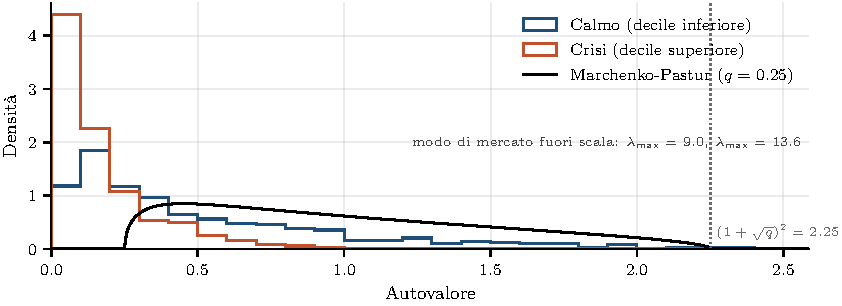
\includegraphics[width=\textwidth]{figures/fig_mp_spectrum.pdf}
\caption[Spettro empirico e legge di Marchenko--Pastur]{Autovalori delle matrici di correlazione nei decili di finestre con la correlazione media più bassa e più alta, confrontati con la densità di Marchenko--Pastur per $q=0{,}250$. In nessuno dei due regimi lo spettro empirico riempie il bulk.}
\label{fig:topo-mp-spectrum}
\end{figure}

\section{Sintesi delle metriche}
\label{sec:topo-orchestration}

Lo script \path{03_topology_analysis.py} applica le funzioni delle sezioni precedenti a tutte le $1947$ finestre e raccoglie i risultati in un unico DataFrame, con una riga per finestra, indicizzata dalla data di chiusura, e una colonna per metrica. La lunghezza dell'MST è calcolata sulle distanze di Mantegna, le due connettività algebriche su $W_{\mathrm{full}}$, connesso in ogni finestra, e la correlazione media e le tre metriche spettrali direttamente su $C_t$. La densità è l'unica calcolata su un grafo filtrato, perché è l'unica che dipende dalla soglia per definizione, ed è riportata, oltre che alla soglia calibrata $\tau$, alla soglia $\tau_{\mathrm{FWER}}=0{,}4311$, più selettiva perché controlla l'errore sull'insieme delle $105$ coppie, e alla soglia fissa $\tau_{\mathrm{fixed}}=0{,}30$. Le due varianti più rade servono a stabilire se un'eventuale serie piatta sia una proprietà del mercato o della soglia.

\begin{table}[H]
\centering
\caption[Metriche topologiche sull'intero periodo]{Statistiche delle metriche topologiche sulle $1947$ finestre mobili.}
\label{tab:topo-summary}
\small
\begin{tabular}{@{}lrrrrr@{}}
\toprule
\textbf{Metrica} & \textbf{Media} & \textbf{Dev. std} & \textbf{Min} & \textbf{Mediana} & \textbf{Max} \\
\midrule
Correlazione media & $0{,}675$ & $0{,}104$ & $0{,}372$ & $0{,}689$ & $0{,}900$ \\
Densità ($\tau$ calibrata) & $0{,}974$ & $0{,}053$ & $0{,}733$ & $1{,}000$ & $1{,}000$ \\
Densità ($\tau_{\mathrm{FWER}}$) & $0{,}887$ & $0{,}129$ & $0{,}371$ & $0{,}924$ & $1{,}000$ \\
Densità ($\tau_{\mathrm{fixed}}$) & $0{,}950$ & $0{,}079$ & $0{,}562$ & $0{,}990$ & $1{,}000$ \\
Connettività algebrica normalizzata & $1{,}024$ & $0{,}022$ & $0{,}923$ & $1{,}028$ & $1{,}058$ \\
Connettività algebrica combinatoria & $7{,}046$ & $1{,}252$ & $3{,}750$ & $7{,}060$ & $10{,}443$ \\
Lunghezza MST normalizzata & $0{,}590$ & $0{,}099$ & $0{,}331$ & $0{,}584$ & $0{,}883$ \\
Entropia spettrale & $1{,}242$ & $0{,}282$ & $0{,}518$ & $1{,}221$ & $2{,}003$ \\
Quota del modo di mercato & $0{,}711$ & $0{,}091$ & $0{,}449$ & $0{,}724$ & $0{,}907$ \\
Autovalori fuori dal bulk & $1{,}004$ & $0{,}064$ & $1{,}000$ & $1{,}000$ & $2{,}000$ \\
\bottomrule
\end{tabular}
\end{table}

Non tutte le serie della \cref{tab:topo-summary} portano lo stesso segnale. La densità alla soglia calibrata ha media $0{,}974$ e mediana $1{,}000$. In più di metà delle finestre nessun arco viene rimosso e il grafo filtrato coincide con quello completo. Alla soglia $\tau_{\mathrm{FWER}}$ la serie varia molto di più (deviazione standard $0{,}129$ contro $0{,}053$). La piattezza è quindi in buona parte un effetto della soglia calibrata, che su un mercato così correlato lascia passare quasi ogni arco.

Le due connettività algebriche si comportano in modo molto diverso. Quella normalizzata resta nell'intervallo $[0{,}923;\,1{,}058]$, con un coefficiente di variazione di $0{,}021$. Quella combinatoria si estende da $3{,}750$ a $10{,}443$, con un coefficiente di variazione di $0{,}178$. La seconda, per questo motivo, compare tra le metriche principali lette attorno alle crisi nella \cref{sec:topo-event-study}.

L'entropia spettrale non supera mai $2{,}003$, ben al di sotto del massimo teorico $\log 15\approx2{,}708$. Una struttura comune ai quindici asset non scompare mai del tutto, nemmeno nella finestra più tranquilla. La quota del modo di mercato quantifica questa struttura. In media il $71\%$ della varianza totale è spiegato dalla sola direzione in cui tutti gli asset si muovono insieme.

Il conteggio degli autovalori fuori dal bulk vale esattamente $1$ in $1939$ finestre su $1947$ e non supera mai $2$. È un risultato distributivo che conferma sui dati dello studio quello di \textcite{laloux1999noise}. Solo il modo di mercato eccede in modo sistematico ciò che il rumore di stima potrebbe produrre da solo.

\section{Il grafo attorno alle crisi}
\label{sec:topo-event-study}

Il periodo di studio include le tre crisi presentate nell'Introduzione: la stretta cinese su scambi e mining del 19/05/2021~\cite{griffith2023cryptocurrency}, il collasso di Terra/Luna del 09/05/2022~\cite{briola2023anatomy} e il fallimento di FTX dell'08/11/2022~\cite{akyildirim2023understanding}. Occorre stabilire se le serie della \cref{sec:topo-orchestration} si muovano in corrispondenza di questi eventi, e con quale intensità rispetto all'intera storia del campione.

\subsection{Offset e percentili}

Il valore alla data $t$ è calcolato sulla finestra di rendimenti $[t-59,\,t]$, quindi alla data dell'evento la finestra termina con il giorno dello shock e i restanti cinquantanove giorni sono tutti precedenti. Lo studio legge perciò ogni metrica a cinque offset dalla data dell'evento, $-60$, $-30$, $0$, $+30$ e $+60$ giorni. L'offset $+60$ è l'unico la cui finestra è interamente successiva all'evento: all'offset $+30$, infatti, la finestra contiene ancora trenta giorni precedenti, cioè metà dei dati. La lettura ai cinque offset è implementata da \texttt{event\_study} in \path{src/cryptognn/events.py}.

\begin{listing}[H]
\begin{minted}{python}
def event_study(
    topology: pd.DataFrame,
    events: list[Event],
    offsets: tuple[int, ...] = DEFAULT_OFFSETS,
) -> pd.DataFrame:
    # Sanity checks on events and offsets, setup of the records list
    ...
    for event in events:
        event_date = pd.Timestamp(event.date)
        for offset in offsets:
            target = event_date + pd.Timedelta(days=offset)
            date_used, values = _read_at(topology, index, target)
            for metric in topology.columns:
                value = values[metric] if values is not None else np.nan
                records.append(
                    {
                        # Event and metric identifiers
                        ...
                        "offset_days": offset,
                        "value": value,
                        "percentile": _percentile(topology[metric], value),
                    }
                )
    study = pd.DataFrame.from_records(records)
    outer = _change_between(study, offsets[0], offsets[-1])
    inner = _change_between(study, offsets[1], offsets[-2]) if len(offsets) >= 4 else pd.Series(np.nan, index=outer.index)
    study["pct_change_clean"] = _broadcast(study, outer)
    study["pct_change_local"] = _broadcast(study, inner)
    return study
\end{minted}
\caption{\texttt{event\_study}}
\label{lst:event-study}
\end{listing}

Il ciclo principale produce una riga per ogni combinazione di evento, offset e metrica. Ogni riga riporta il valore letto e il suo percentile, cioè la frazione dell'intero campione di $1947$ finestre strettamente inferiore a quel valore. Il percentile rende confrontabili metriche su scale diverse. La correlazione media vive in $[0,1]$, la connettività combinatoria tra $3{,}75$ e $10{,}44$, ma un valore al $99$\textdegree{} percentile ha lo stesso significato per entrambe. Un offset che cade fuori dal campione restituisce un valore mancante invece della data disponibile più vicina, che potrebbe distare mesi. A valle del ciclo, le variazioni percentuali sono calcolate da \texttt{\_change\_between}.

\begin{listing}[H]
\begin{minted}{python}
def _change_between(study: pd.DataFrame, start_offset: int, end_offset: int) -> pd.Series:
    pivot = study.pivot_table(
        index=["event_key", "metric"], columns="offset_days", values="value", dropna=False
    )
    return 100.0 * (pivot[end_offset] - pivot[start_offset]) / pivot[start_offset]
\end{minted}
\caption{\texttt{\_change\_between}}
\label{lst:change-between}
\end{listing}

La tabella pivot riorganizza le righe prodotte dal ciclo, con una riga per ogni coppia di evento e metrica e una colonna per ogni offset. L'istruzione \texttt{return} calcola, per ogni coppia, la variazione percentuale del valore $x$ della metrica tra due offset $a$ e $b$:
\begin{equation}
    \Delta_{a\to b} = 100\cdot\frac{x_b-x_a}{x_a}.
    \label{eq:pct-change}
\end{equation}
La variazione principale, $\Delta_{-60\to+60}$, confronta la finestra interamente precedente all'evento con quella interamente successiva. La secondaria, $\Delta_{-30\to+30}$, è tra gli offset interni ed è definita solo quando gli offset sono almeno quattro.

\subsection{Risultati}

La \Cref{tab:topo-event-china} riporta le metriche attorno alla stretta cinese a $-60$, $0$ e $+60$ giorni, con la variazione $\Delta_{-60\to+60}$ e il percentile a $+60$ giorni.

\begin{table}[H]
\centering
\caption[Metriche attorno alla stretta cinese]{Metriche topologiche attorno alla stretta cinese (19/05/2021)~\cite{griffith2023cryptocurrency}. La colonna \%+60g riporta il percentile a $+60$ giorni.}
\label{tab:topo-event-china}
\begin{tabular*}{\textwidth}{@{\extracolsep{\fill}}lrrrrr@{}}
\toprule
\textbf{Metrica} & \textbf{$\mathbf{-60}$g} & \textbf{0g} & \textbf{+60g} & $\mathbf{\Delta_{-60\to+60}}$ & \textbf{\%+60g} \\
\midrule
Corr. media & $0{,}430$ & $0{,}611$ & $0{,}868$ & $+101{,}8\%$ & $99{,}4\%$ \\
Densità ($\tau$) & $0{,}848$ & $0{,}971$ & $1{,}000$ & $+18{,}0\%$ & $36{,}0\%$ \\
Densità ($\tau_{\mathrm{FWER}}$) & $0{,}438$ & $0{,}790$ & $1{,}000$ & $+128{,}3\%$ & $72{,}9\%$ \\
Connett. comb. & $5{,}284$ & $6{,}254$ & $9{,}848$ & $+86{,}4\%$ & $99{,}3\%$ \\
Lunghezza MST & $0{,}826$ & $0{,}654$ & $0{,}386$ & $-53{,}3\%$ & $0{,}5\%$ \\
Entropia spettrale & $1{,}873$ & $1{,}418$ & $0{,}652$ & $-65{,}2\%$ & $0{,}5\%$ \\
Modo di mercato & $0{,}499$ & $0{,}658$ & $0{,}878$ & $+76{,}0\%$ & $99{,}4\%$ \\
\bottomrule
\end{tabular*}
\end{table}

La \Cref{tab:topo-event-china} omette la densità a soglia fissa $\tau_{\mathrm{fixed}}$, ridondante con le altre due, la connettività normalizzata perché pressoché piatta e il conteggio degli autovalori fuori dal bulk, che vale $1$ ad ogni offset. Il valore $1{,}000$ è il massimo possibile per la densità a $+60$ giorni, ma il percentile conta solamente le finestre con valore strettamente inferiore. Poiché il $64\%$ delle finestre ha densità esattamente pari a $1$, un grafo saturo si colloca al $36$\textdegree{} percentile.

La stretta cinese rappresenta il caso caratteristico del compattamento descritto nella \cref{sec:topo-measuring-compaction}: la correlazione media raddoppia tra le due finestre disgiunte, la connettività combinatoria sale dell'$86{,}4\%$ e la quota del modo di mercato del $76{,}0\%$. Ogni metrica si muove nella direzione attesa e quasi ognuna raggiunge un estremo della propria distribuzione storica. La \cref{fig:topo-china} ritrae la finestra a $+60$ giorni. Alla soglia calibrata il grafo è completo, compattamento osservabile nello spessore degli archi e nella matrice di correlazione.

\begin{figure}[H]
\centering
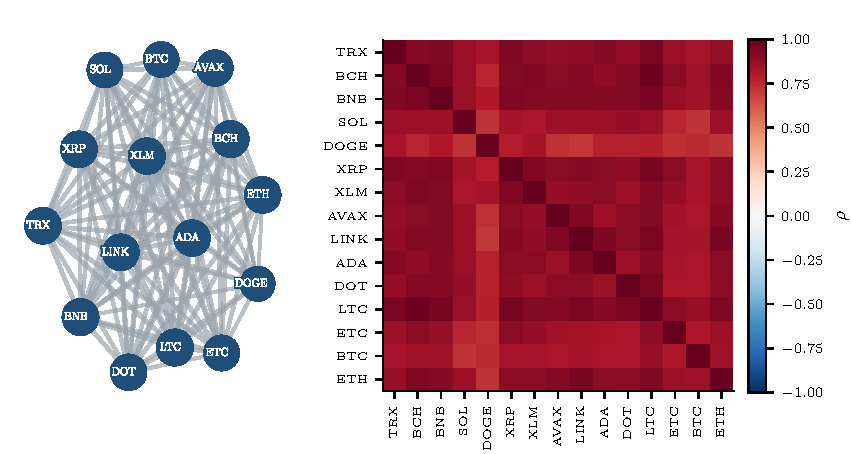
\includegraphics[width=\textwidth]{figures/fig_event_china_crackdown.pdf}
\caption[Grafo e correlazioni a $+60$ giorni dalla stretta cinese]{Finestra a $+60$ giorni dalla stretta cinese (18/07/2021). A sinistra il grafo filtrato $W_{\mathrm{thresh}}$, con lo spessore di ogni arco proporzionale al peso e la dimensione di ogni nodo al grado pesato; le posizioni dei nodi sono calcolate una sola volta sul grafo medio dell'intero periodo e riusate in tutte e tre le figure di evento. A destra la matrice di correlazione $C_t$ della stessa finestra, con gli asset ordinati per clustering gerarchico e la scala del colore fissata a $[-1,1]$.}
\label{fig:topo-china}
\end{figure}

\begin{table}[H]
\centering
\caption[Metriche attorno a Terra/Luna e FTX]{Variazione $\Delta_{-60\to+60}$ e percentile a $+60$ giorni per Terra/Luna (09/05/2022)~\cite{briola2023anatomy} e FTX (08/11/2022)~\cite{akyildirim2023understanding}.}
\label{tab:topo-event-terra-ftx}
\begin{tabular*}{\textwidth}{@{\extracolsep{\fill}}lrrrr@{}}
\toprule
 & \multicolumn{2}{c}{\textbf{Terra/Luna}} & \multicolumn{2}{c}{\textbf{FTX}} \\
\cmidrule(lr){2-3}\cmidrule(lr){4-5}
\textbf{Metrica} & $\mathbf{\Delta_{-60\to+60}}$ & \textbf{\%+60g} & $\mathbf{\Delta_{-60\to+60}}$ & \textbf{\%+60g} \\
\midrule
Corr. media & $-1{,}1\%$ & $86{,}7\%$ & $+7{,}0\%$ & $91{,}6\%$ \\
Densità ($\tau$) & $0{,}0\%$ & $36{,}0\%$ & $0{,}0\%$ & $36{,}0\%$ \\
Densità ($\tau_{\mathrm{FWER}}$) & $-1{,}9\%$ & $62{,}5\%$ & $0{,}0\%$ & $72{,}9\%$ \\
Connett. comb. & $-20{,}2\%$ & $64{,}7\%$ & $+6{,}1\%$ & $95{,}5\%$ \\
Lunghezza MST & $-1{,}8\%$ & $14{,}6\%$ & $-15{,}9\%$ & $13{,}0\%$ \\
Entropia spettrale & $-2{,}9\%$ & $12{,}2\%$ & $-17{,}8\%$ & $11{,}5\%$ \\
Modo di mercato & $-0{,}3\%$ & $87{,}1\%$ & $+6{,}5\%$ & $90{,}2\%$ \\
\bottomrule
\end{tabular*}
\end{table}

Le due crisi del 2022 presentano un quadro diverso (\cref{tab:topo-event-terra-ftx}). La densità alla soglia calibrata vale $1{,}000$ a tutti e cinque gli offset, per entrambi gli eventi. Il grafo filtrato era quindi già completo prima dello shock e non aveva margine per compattarsi ulteriormente. Le variazioni delle altre metriche sono contenute. Per FTX vanno tutte nella direzione del compattamento, con ampiezze tra il $6\%$ e il $18\%$. Per Terra/Luna i segni sono misti e la connettività combinatoria scende del $20{,}2\%$. I percentili forniscono però un'importante lettura. A $+60$ giorni da entrambi gli eventi la correlazione media e la quota del modo di mercato si collocano sopra l'$85$\textdegree{} percentile, l'entropia spettrale e la lunghezza dell'MST sotto il $15$\textdegree{}. Il mercato si trovava in uno stato di forte compattamento, anche prima degli eventi. A $-60$ giorni la correlazione media valeva $0{,}799$ per Terra/Luna e $0{,}753$ per FTX, contro una media storica di $0{,}675$. Nel 2022 la struttura del mercato era quindi già vicina alla saturazione, e una crisi può spostare di poco metriche che si trovano già vicino al proprio estremo. Le \cref{fig:topo-terra-luna,fig:topo-ftx} ritraggono le finestre a $+60$ giorni dei due eventi: grafi completi come quello della stretta cinese e matrici sature nella stessa misura, a dodici e a diciotto mesi di distanza.

\begin{figure}[H]
\centering
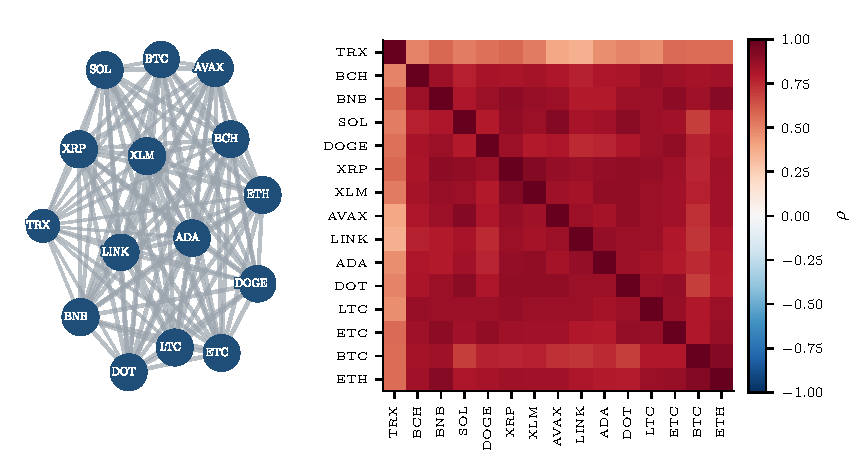
\includegraphics[width=\textwidth]{figures/fig_event_terra_luna.pdf}
\caption[Grafo e correlazioni a $+60$ giorni da Terra/Luna]{Finestra a $+60$ giorni dal collasso di Terra/Luna (08/07/2022), disegnata come la \cref{fig:topo-china}: grafo filtrato a sinistra, matrice di correlazione a destra, stesse posizioni dei nodi e stesso ordinamento degli asset.}
\label{fig:topo-terra-luna}
\end{figure}

\begin{figure}[H]
\centering
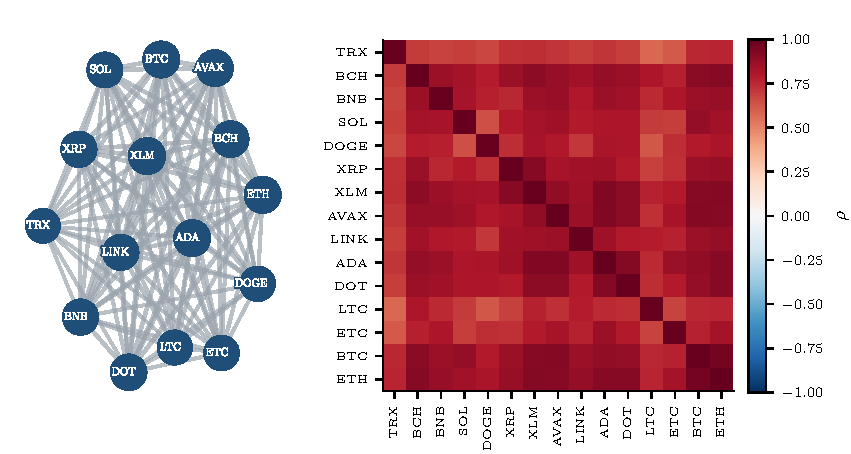
\includegraphics[width=\textwidth]{figures/fig_event_ftx.pdf}
\caption[Grafo e correlazioni a $+60$ giorni dal fallimento di FTX]{Finestra a $+60$ giorni dal fallimento di FTX (07/01/2023), disegnata come la \cref{fig:topo-china}.}
\label{fig:topo-ftx}
\end{figure}

La \Cref{fig:topo-timeseries} riassume l'intero periodo, con quattro delle serie sulle $1947$ finestre e le tre date di crisi sovrapposte. L'asse temporale è condiviso, così che la linea verticale di un evento si legga su tutti i pannelli contemporaneamente. Dopo la stretta cinese ogni pannello mostra un salto netto, mentre le linee di Terra/Luna e FTX cadono su serie già vicine ai propri estremi.

\begin{figure}[H]
\centering
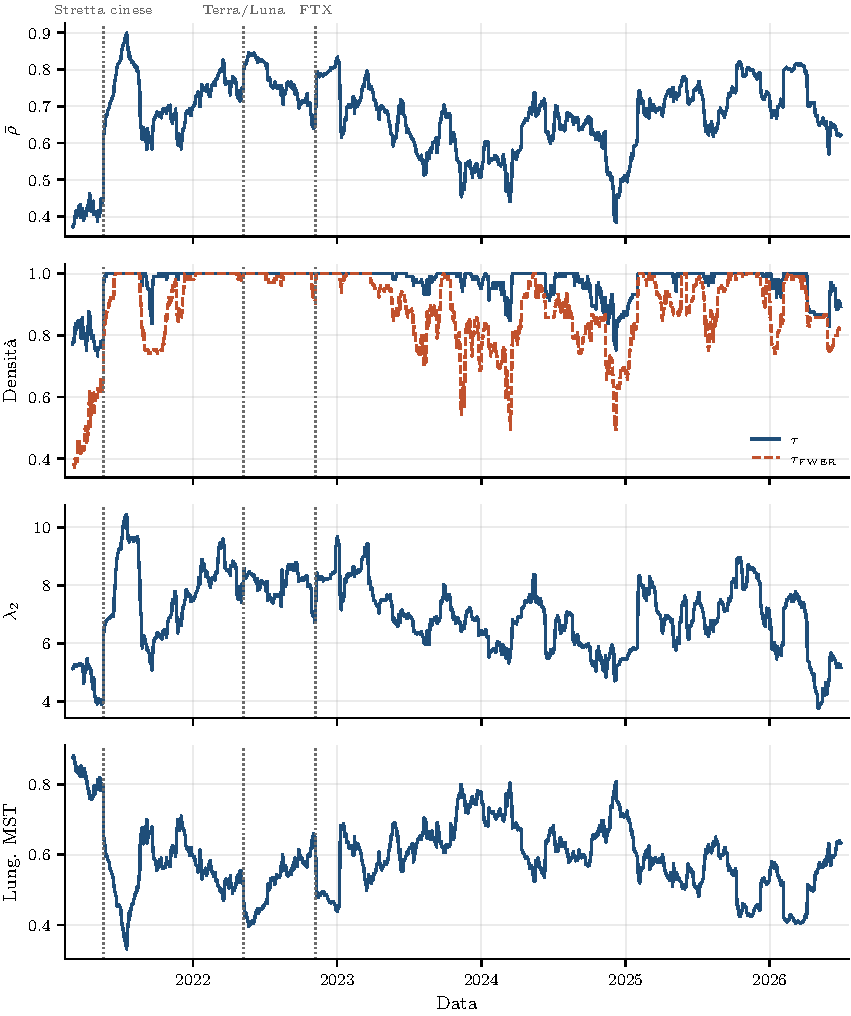
\includegraphics[width=\textwidth]{figures/fig_topology_timeseries.pdf}
\caption[Serie temporali delle metriche topologiche]{Correlazione media, densità alle soglie $\tau$ e $\tau_{\mathrm{FWER}}$, connettività algebrica combinatoria e lunghezza normalizzata dell'MST sulle $1947$ finestre dell'intero periodo, con le date dei tre eventi di crisi sovrapposte a ogni pannello.}
\label{fig:topo-timeseries}
\end{figure}
